\section{REST-API}
In diesem Projekt werden API-Endpunkte (gekapselt in sog. \emph{Controllern}) und andere Funktionen wie z.\,B. Datenbankoperationen voneinander getrennt.
Das verwendete HTTP-Framework bindet den HTTP-Request an eine Funktion, wodurch eine einfache und saubere Implementierung ermöglicht wird.
Somit können Endpunkte einfach verschoben und Integration Tests einfacher durchgeführt werden.
Annotationen mit den HTTP-Verben definieren dabei die Art der Anfrage.
Das ermöglicht, die Zugehörigkeit direkt im Quelltext abzulesen.

Die in der URL übertragenen Parameter werden direkt die der Funktion zugeordnet.
Dadurch wird sichergestellt, das die Daten aus dem Body der Anfrage dem Datentyp entsprechen, den die Funktion verarbeiten kann.
Sollte dies nicht der Fall sein, beantwortet das Framework, welches in Abschnitt \ref{backend} genauer erklärt wird, die Anfrage mit einem HTTP-Fehlercode.

Funktion geben immer ein \texttt{IActionResult} zurück, welches die Klasse \linebreak\texttt{ObjectResult} enthält.
Die hier am Wichtigsten enthaltenen Eigenschaften sind der Statuscode und der Body.
Das Framework kann somit eine HTTP-Antwort zurückgeben und gleichzeitig können Integration Tests intern, d.\,h. ohne HTTP, durchgeführt werden.
\linebreak
\linebreak
Eine Übersicht aller verfügbaren Controller ist in den Tabellen \vref{controller1} und \vref{controller2} zu finden. Zu beachten ist, dass alle Endpunkte zusätzlich zu den angegeben Statuscodes auch die Codes \texttt{401 Unauthorized} oder \texttt{403 Forbidden} bei fehlender Authentifizierung und \texttt{500 Internal Server Error} bei einer Systemfehlkonfiguration zurückgeben können.
\linebreak
\linebreak
Der nicht erwähnte Endpunkt \texttt{/Authentication/register-admin} wird benötigt, um ein Administratorkonto anzulegen.
Daher wird er nur zur Einrichtung des Systems benötigt um MUSS aus Sicherheitsgründen anschließend durch eine Firewall, \texttt{.htaccess}-Datei o.ä. blockiert werden.
Methode, Rollen, Parameter, Rückgabe und Statuscodes sind identisch mit \texttt{/Authentication/register}.

Werden Benutzerkonten von einem Administrator zentral verwaltet, sollte der Endpunkt zur Registrierung ebenso abgesichert werden.

\begin{sidewaystable}
	\caption{Controller Definitionen 1/2}
	\centering
	\label{controller1}
\begin{tabular}{llllllll}
	Controller   & Name          & Methode & Rolle     & URL       & Parameter          & Rückgabe                          & Statuscodes   \\
	Product      & GetProducts   & GET     & Seller    & /all      & null               & List\textless{}uint\textgreater{} & 200, 404      \\
	Product      & GetProduct    & GET     & Seller    & /\{id\}   & uint id            & Product                           & 200, 404      \\
	Product      & AddProduct    & POST    & Manager   & /add      & Product p          & Product                           & 201, 409      \\
	Product      & ModifyProduct & PUT     & Manager   & /\{id\}   & uint id, Product p & Product                           & 200, 404, 423 \\
	Product      & DeleteProduct & DELETE  & Manager   & /\{id\}   & uint id            & null                              & 200, 404, 423 \\
	&               &         &           &           &                    &                                   &               \\
	Price        & GetPrices     & GET     & Admin     & /all      & null               & List\textless{}Guid\textgreater{} & 200, 404      \\
	Price        & GetPrice      & GET     & Manager   & /\{id\}   & Guid id            & Price                             & 200, 404      \\
	Price        & AddPrice      & POST    & Manager   & /add      & Price p            & Price                             & 201, 409      \\
	Price        & ModifyPrice   & PUT     & Manager   & /\{id\}   & Guid id, Price p   & Price                             & 200, 404, 423 \\
	Price        & DeletePrice   & DELETE  & Manager   & /\{id\}   & Guid id            & null                              & 200, 404, 423 \\
	&               &         &           &           &                    &                                   &               \\
	Group        & GetGroups     & GET     & Manager   & /all      & null               & List\textless{}Guid\textgreater{} & 200, 404      \\
	Group        & GetGroup      & GET     & Manager   & /\{id\}   & Guid id            & Group                             & 200, 404      \\
	Group        & AddGroup      & POST    & Manager   & /add      & Price p            & Group                             & 201, 409      \\
	Group        & ModifyGroup   & PUT     & Manager   & /\{id\}   & Guid id, Price p   & Group                             & 200, 404, 423 \\
	Group        & DeleteGroup   & DELETE  & Manager   & /\{id\}   & Guid id            & null                              & 200, 404, 423 \\
	&               &         &           &           &                    &                                   &               \\
	Authenticate & Login         & POST    & Anonymous & /login    & LoginModel l       & string                            & 200           \\
	Authenticate & Register      & POST    & Anonymous & /register & RegisterModel r    & bool                              & 200           \\
	&               &         &           &           &                    &                                   &               \\
	Misc         & Ping          & GET     & Anonymous & /ping     & null               & "Pong"                            & 200          
\end{tabular}
\end{sidewaystable}

\begin{sidewaystable}
	\caption{Controller Definitionen 2/2}
	\centering
	\label{controller2}
\begin{tabular}{llllllll}
	Controller & Name             & Methode & Rolle   & URL             & Parameter      & Rückgabe                                & Statuscodes \\
	Purchase   & GetPurchases     & GET     & Seller  & /all            & null           & List\textless{}Guid\textgreater{}       & 200, 404    \\
	Purchase   & GetPurchase      & GET     & Seller  & /\{id\}         & uint id        & Purchase                                & 200, 404    \\
	Purchase   & SellPurchase     & POST    & Seller  & /sell           & Purchase p     & Guid                                    & 200         \\
	Purchase   & BuyPurchase      & POST    & Seller  & /buy            & Purchase p     & Guid                                    & 200         \\
	Purchase   & CancelPurchase   & POST    & Seller  & /cancel         & Purchase p     & Guid                                    & 200         \\
	Purchase   & RefundPurchase   & POST    & Seller  & /refund         & Purchase p     & Guid                                    & 200         \\
	Purchase   & DisposalPurchase & POST    & Manager & /dispose        & Purchase p     & Guid                                    & 200         \\
	&                  &         &         &                 &                &                                         &             \\
	Stats      & GetTotalStats    & GET     & Analyst & /total          & null           & List\textless{}TotalStats\textgreater{} & 200, 204    \\
	Stats      & GetYearStats     & GET     & Analyst & /year/\{i\}     & ushort i       & YearStats                               & 200, 404    \\
	Stats      & GetAllYearStats  & GET     & Analyst & /year/all       & null           & List\textless{}ushort\textgreater{}     & 200, 204    \\
	Stats      & GetMonthStats    & GET     & Analyst & /month/y/m      & ushort y, m    & MonthStats                              & 200, 404    \\
	Stats      & GetAllMonthStats & GET     & Analyst & /month/all      & null           & List\textless{}DateTime\textgreater{}   & 200, 204    \\
	Stats      & GetDayStats      & GET     & Analyst & /day/y/m/d      & ushort y, m, d & DayStats                                & 200, 404    \\
	Stats      & GetAllDayStats   & GET     & Analyst & /day/all        & null           & List\textless{}DateTime\textgreater{}   & 200, 204    \\
	Stats      & GetProductStats  & GET     & Analyst & /product/\{id\} & uint id        & ProductStats                            & 200, 404   
\end{tabular}
\end{sidewaystable}

\newpage
\section{Weitere Bestandteile}
Die API basiert hauptsächlich auf dem Framework \texttt{Microsoft.Entity\-Framework\-Core}.
Ein Objekt vom Typ \texttt{IHost} (Host) mit einer \texttt{IConfiguration} (Konfiguration) schafft die Grundlage der API.
Welche API-Controller eingebunden sind, die Anbindung der Datenbank sowie die Definition der Zugriffsrechte sind Informationen, die in der Konfiguration enthalten sind.

Das bereits im Framework eingebaute Werkzeug \emph{SwaggerUI} kann verwendet werden, um den Aufbau der API grafisch darzustellen und Anfragen direkt über den Browser stellen zu können.
Hier werden auch Definitionen, Kommentare und Datentypen beschrieben und wie sie in der API verwendet werden können.

\subsection{Datenbank}
Das verwendete Datenbanksystem ist SQLite.
Benutzer und Anwendungsdaten werden in zwei getrennten .db-Dateien gespeichert.
Der Grund für diese Trennung liegt in der Funktionsweise der Anbindung.
Während für die Datenbank mit den Anwendungsdaten ein Klasse vom Typ \texttt{DbContext} verwendet wird, benötigt die Verarbeitung der Benutzer und Rollen einen \texttt{IdentityDbContext}.

Damit es hier nicht zu Migrationsproblemen kommt und die Benutzerdaten bei einer Änderung der Datenstruktur nicht erneut generiert werden müssen, wurden die beiden Kontext-Klassen nicht zusammengelegt.
Außerdem macht diese Methode es möglich, Anwendungsdaten und Benutzerdaten an getrennten Orten aufzubewahren, was im Sinne der Datensicherheit und des Datenschutzes ist.

Die Klassen für Benutzer- und Rollendaten werden von den beiden Frameworks \texttt{Microsoft.\-AspNetCore\-.Identity} und \texttt{Microsoft.\-AspNetCore.\-Identity.\linebreak\-Entity\-Framework\-Core} bereitgestellt. 
Die Eigenschaften und Beziehungen der Anwendungsdaten können Abbildung \vref{data-erm} entnommen werden.

\subsection{Authentifizierung}
Damit Endpunkte verwendet werden können, muss sich der Benutzer dafür authentifizieren. 
Dieser Vorgang wird in Abbildung \vref{login-struct} beschrieben.
Die Endpunkte zum Registrieren und Anmelden sind Anonym erreichbar.
Im Body der Anfrage muss ein JSON-Objekt mitgegeben werden, welches entweder von der Klasse LoginModel oder RegisterModel abstammt.
Zweiteres enthält zusätzlich zu den Eigenschaften Username und Password des LoginModel eine Zeichenkette für die E-Mail Adresse des Benutzers.

Ist eine Anmeldung erfolgreich gewesen, sendet der Server eine Antwort mit einem JWT im Body.
Diesen muss der Client bei allen anderen Anfragen im Authorization-Header mitsenden, um vom Server Authentifiziert zu werden.

\begin{figure}[ht]
	\centering
	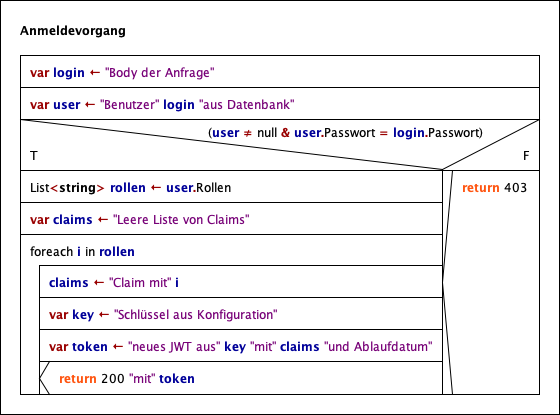
\includegraphics[width=0.7\linewidth]{Anmeldevorgang.png}
	\caption{Ablauf der Anmeldung}
	\label{login-struct}
\end{figure}

\begin{figure}[ht]
	\centering
	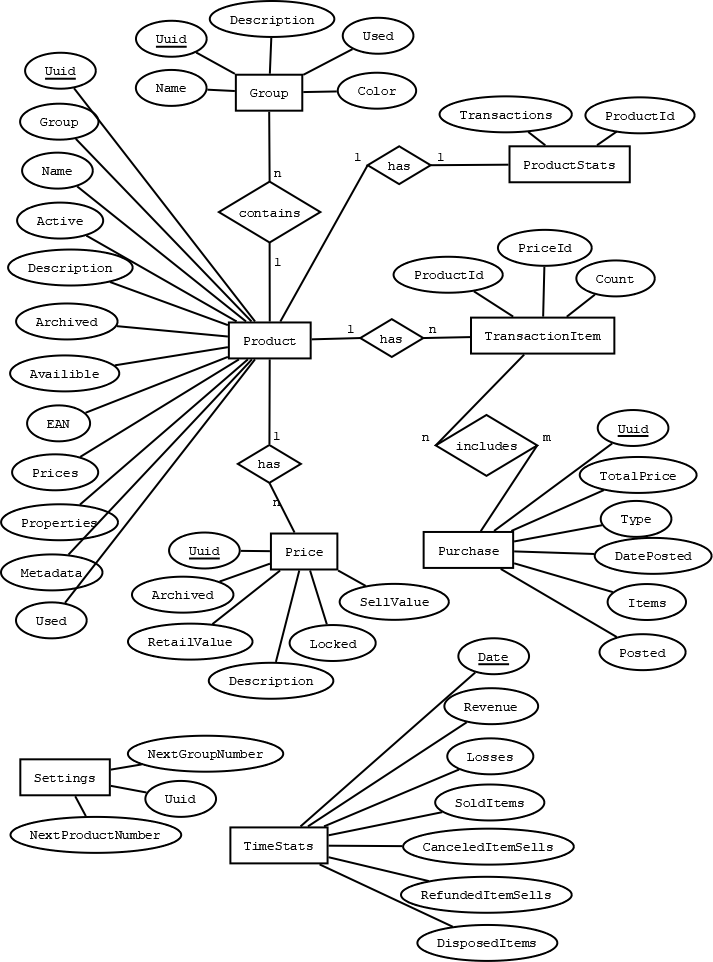
\includegraphics[width=1\linewidth]{ERM.png}
	\caption{ERM der Anwendungsdaten}
	\label{data-erm}
\end{figure}

\subsection{Verarbeitung von Anfragen}
Empfangene Anfragen werden nach einer Prüfung der Identität des Clients an den zuständigen Controller geleitet, der den angesprochenen Endpunkt enthält.
Demonstriert wird dieser Vorgang in Abbildung \vref{product-creation} anhand der Erstellung eines Produkts.

Die Kommunikation zwischen Datenbank und API findet über einen \texttt{DbContext} statt.
Dieser ermöglicht es, die verwendeten Klassen der Objekte direkt in Tabellen zu konvertieren, damit diese mit einem Befehl abgerufen und manipuliert werden können. Daher sind in der API kein vorgeschriebenen SQL-Abfragen vorhanden.

Nach Beendung der Bearbeitung der Datenbank erzeugt jeder Endpunkt ein HTTP-Fähiges Resultat, welches über den Controller an den Client zurückgegeben wird.
Eine genaue Definition der Rückgaben aller Endpunkte ist in den Tabellen \vref{controller1} und \vref{controller2} zu finden.
 
\begin{sidewaysfigure}[ht]
	\centering
	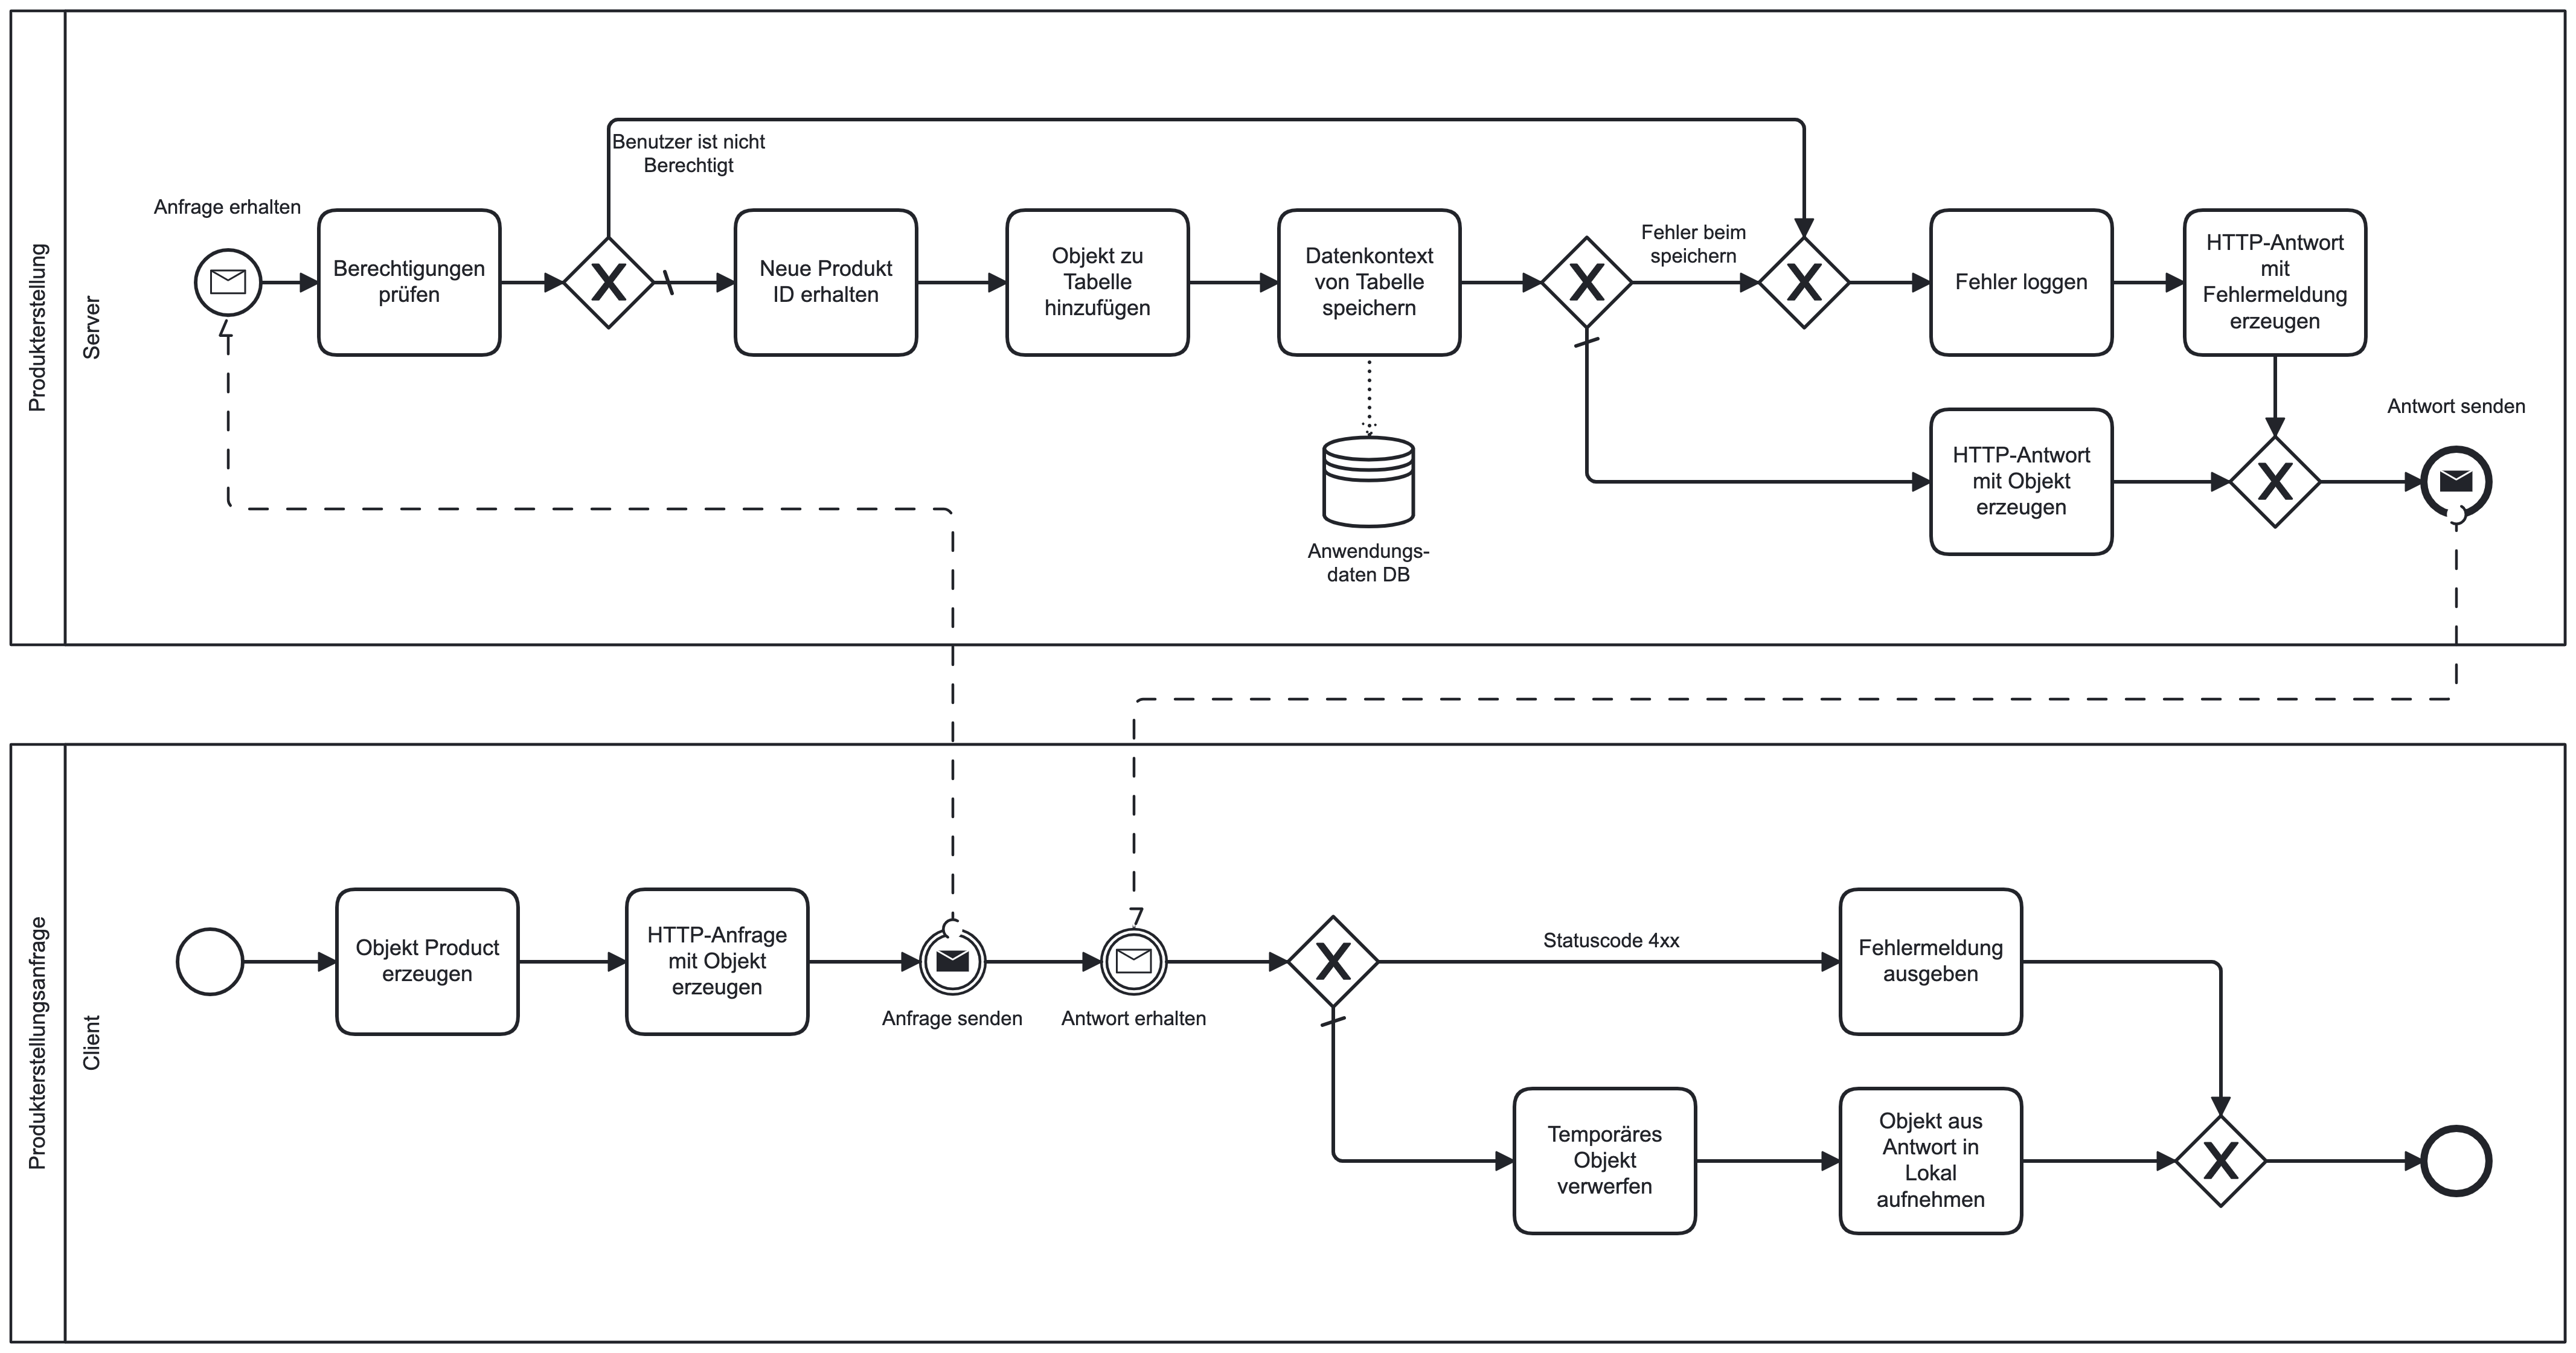
\includegraphics[width=1\linewidth]{Produkterstellung.png}
	\caption{Ablauf der Anmeldung}
	\label{product-creation}
\end{sidewaysfigure}